
\section{Lepton identification}
The following three sections briefly describe how certain subsystems of the CMS detector work together to identify muons, electrons, and tau leptons. 

\subsection{Muon identification systems}

As CMS implies in its name, muons are certainly a focal point in particle detection. 
Looking at muons that come from the interaction vertex---prompt muons---the tracker plays an important role in identifying charged particle tracks. 
The tracker system works in conjunction with the gas chambers to reconstruct muons, and the solenoid bends the muon's tracks allowing the momentum to be measured for an accurate mass resolution. By design, muons should be the only particle that should reach the gas chambers, making for great muon efficiency. 
During reconstruction, muons are identified and are ultimately divided into four working points (very loose, loose, medium, tight). These points are defined based on their efficiencies and depend on the $\chi^2$ of the track and momentum of the candidate muon ~\cite{CMS-PAS-PFT-09-001,Kratschmer:1956760}.


\subsection{Electron identification systems}
The main subdetector involved with electron identification is the ECAL. To identify electrons, a cluster of energy in the ECAL is associated with a track that is constructed in the silicon detector system. 
The tracks are identified in the typical fashion using the Kalman Filter tracking technique to pick good quality tracks, and then the tracks are refitted using a Gaussian Sum Filter. 
These tracks are then associated with an ECAL super cluster---grouped energy deposits---by requiring matching in $\eta,\;\phi$ space
\begin{equation}|\Delta\eta| = |\eta_{\text{SC}} - \eta_{\text{in}}^{\text{extrap}}| < 0.02\end{equation}
\begin{equation}|\Delta\phi| = |\phi_{\text{SC}} - \phi_{\text{in}}^{\text{extrap}}| < 0.15\end{equation}
This method has an overall efficiency of about 93\% ~\cite{Khachatryan:2015hwa}. 

\subsection{Tau identification systems}
Tau leptons decay in many different ways. It is the heaviest lepton, so heavy it can decay to intermediate mesons such as the $\rho$, $a$, and $\pi$ mesons.
Ergo, when it comes to tau identification, many algorithms are needed to properly identify them using information across the detector. 
Tau leptons decay both hadronically and leptonically as shown in the table \ref{tab:taudecay} below. 



\begin{table}[h!tbp]
\centering
    \topcaption{Possible hadronic tau decays, $h$ doesn't indicate a Higgs particle but a hadronic prong~\cite{Workman:2022}}
\label{tab:taudecay}
\begin{tabular}{c c r}
Decay Modes & Resonance & \multicolumn{1}{c}{$\mathcal{B}(\%)$} \\\hline
Leptonic Decay && \multicolumn{1}{l}{35.2}\\
$\tau^- \rightarrow e^- \bar{\nu}_e \nu_\tau $ & & 17.8 \\
$\tau^- \rightarrow \mu^- \bar{\nu}_\mu \nu_\tau$ & & 17.4 \\\hline
Hadronic Decay && \multicolumn{1}{l}{64.8}\\
$\tau^- \rightarrow h^-\nu_\tau$ & & 11.5 \\
$\tau^- \rightarrow h^-\pi^0 \nu_\tau$ & $\rho(770)$ & 25.9 \\
$\tau^- \rightarrow h^-\pi^0 \pi^0 \nu_\tau$ & $a_1(1260)$ & 9.5 \\
$\tau^- \rightarrow h^- h^+ h^- \nu_\tau$ & $a_1(1260)$ & 9.8 \\
$\tau^- \rightarrow h^- h^+ h^- \pi^0 \nu_\tau$ & & 4.8 \\
Other & & 3.3 \\\hline
\end{tabular}
\end{table}

%The important algorithms directly related to hardware are the Hadron Plus Strips (HPS) algorithm which combines the use of the tracker system and the electromagnetic calorimeter (ECAL) for hadronic tau identification ~\cite{Sirunyan_2018}.  

The Hadron Plus Strips (HPS) combines the use of the tracker system and the electromagnetic calorimeter (ECAL) for hadronic tau identification ~\cite{Sirunyan_2018}.  


 


\section{Data and simulation}
For this analysis, muons are paramount, so there must be a certain number of muons triggered for the event to be selected. Two final states contain electrons, so datasets containing electrons are also used. The single muon, double muon, and electron plus photon datasets are used depending on the year. These datasets contain the triggers that are the most important for object selection. Single muon triggers that contain isolated muons at 22, 24, and 27 GeV thresholds are implemented, along with double muon triggers with good reconstructed muons at a 17 GeV threshold. More information on triggers and selection is given in the event selection section ~\ref{sec:trig}. 

The simulation typically used to compare with data is MadGraph5@NLO with PYTHIA 8 for hadronization \cite{PYTHIA}. These CMS centrally-generated samples are then digitized using GEANT4 \cite{GEANT4} to the same format as real data events collected and processed at CMS HLT. This raw data is then reconstructed to physics objects---such as tracks and higher level objects like leptons. A direct comparison between data and simulation can be made after calibrating simulation in control regions. 

Data taken from CMS during the entire Run II period was examined, corresponding to 137 $\text{fb}^{-1}$ of integrated luminosity. The list of data and simulation Monte Carlo (MC) is exhaustive and listed in the appendix \ref{app:data}.   

For the MC production of the signal samples, to reflect the 2HDM modeling, events were generated at tree level for a pseudoscalar Higgs like boson between the masses of 15 and 60 GeV in intervals of 5 GeV with the parent Higgs produced through gluon fusion. These masses are sufficient for the parametric modeling, which is used in the fit model, to obtain a precise peak resolution ~\ref{sec:fitmodel}. Signal samples were produced centrally by CMS for 2016, but privately produced for 2017 and 2018. The scripts and conditions used are located here:\\
 \texttt{https://github.com/samhiggie/iDM-analysis-AODproducer/tree/haa} .\\
The NMSSMHET model was used to simulate the events. Parameters and information can be seen in the package:
https://cms-project-generators.web.cern.ch/cms-project-generators/ .



\section{Physics object selection} 
\label{sec:objsel}
%Baseline selections are recommended by the various Physics Object Groups (POGs) for object selection. Ultimately, these take the form of cuts for leptons based primary on kinematic variables like the momentum. 
Baseline selections for objects are recommended by the various Physics Object Groups (POGs). The process of making selections on variables is known as ``making cuts". Ultimately, these take the form of cuts for leptons based primary on kinematic variables like the momentum. 
Selections are made to identify muons, electrons, and tau leptons. These three leptons form the objects under selection and comprise the final states in the analysis.
All leptons under consideration must pass trigger requirements that depend on momentum of the lepton. Special triggers are used for the different final states depending on the number of muons in the event. A precise description of the triggers used are given later in section ~\ref{sec:trig}.
Identifying particles in object selection is critical, particularly differentiating between lepton candidates that come from the interaction vertex (prompt) and those that appear from decays down the line (nonprompt). Relative isolation is typically defined in order to ensure there is no overlap between candidate leptons, to make sure that each lepton is not associated with other physics objects like jets. More details on this variable and it's usage in the Particle Flow algorithm can be found here  ~\cite{Sirunyan_2017}. 
\begin{equation}
I^{\ell} \equiv \frac{\sum_\text{charged}  \PT + \max\left( 0, \sum_\text{neutral}  \PT
                                         - \frac{1}{2} \sum_\text{charged, PU} \PT  \right )}{\PT^{\ell}}.
\label{eq:reconstruction_isolation}
\end{equation}
$\sum_\text{charged}  \PT$ is the scalar sum of the
transverse momenta of the charged particles originating from
the primary vertex and contained in a cone of size
$\Delta R = \sqrt{\smash[b]{(\Delta \eta)^2 + (\Delta \phi)^2}} = 0.4$\,(0.3)
centered on the muon (electron) direction. The sum $\sum_\text{neutral}  \PT$ is
a similar quantity for neutral particles. Track association isn't possible with neutral particles and thus not with primary vertex information; therefore, to take pileup into consideration, an estimate of the transverse momentum from the pile up contribution is subtracted (PU $\PT$).  

As mentioned in the instrumentation and detector chapter~\ref{chap:cmsdet}, the muon identification system uses the tracker to identify charged tracks and the muon chambers to identify the particles later in their trajectory after they exit the solenoid. Typically, ``good" muons are those that are both associated with a track and their subsequent identification in the drift tubes, CSCs, or RPCs. The average muon lifetime is 2.2 $\mu$s so they travel quite far from the interaction point.  The physics object group's recommendations are followed, which select muons with $\pt>15\GeV$ and $\abs{\eta}<2.4$ in addition to selecting only ``good" muons.

Electrons originating from the tau decay are reconstructed by track association along with energy deposition in the Electronic Calorimeter (ECAL). Events are vetoed for candidate electrons that also show a substantial energy deposition in the HCAL for better efficiency. The hits and track quality from two separate algorithms, along with the geometrical and energy matching from the ECAL are used in a Multivariate Analysis (MVA) technique to select good electrons for analysis 
~\cite{Khachatryan:2015hwa}.

To identify $\tauh$ candidates, the hadron-plus-strips (HPS) algorithm is used to identify the major modes of the hadronic tau decay ~\cite{Sirunyan_2018}. Typically, events with hadronic prongs---charged hadrons---are considered in combination with a number of neutral pions and missing transverse energy from the neutrinos. Neutral pions almost always decay to photons, so a hadronic tau identification algorithm should combine the identification of charged hadrons and neutral pions. 
The hadron plus strips (HPS) algorithm combines inner track information, hits in the HCAL, and pion association in the ECAL by deposits in a $\eta,\phi$ strip region to identify hadronic tau leptons. 
The $\tauh$ is matched to $h^{\pm}$, $h^{\pm}\pi^{0}$, $h^{\pm}h^{\mp}h^{\pm}$, or $h^{\pm}h^{\mp}h^{\pm}\pi^{0}$ depending on the overall charge vs neutral constituents ~\cite{Sirunyan:2018pgf,Hassanshahi:2797703}.
In addition to the HPS algorithm, a Deep Neural Network (DNN) was constructed to further aid in identification by discriminating between genuine tau leptons and those that originate from quarks or gluon jets, electrons, or muons.  
In the DNN, the tau four-momentum and charge,
the number of charged and neutral particles constituents,
the isolation variables,
the compatibility of the leading tau track with the primary vertex,
the properties of a secondary vertex in case of a multiprong tau decay,
observables related to the $\eta$ and $\phi$ distributions of energy reconstructed in the ECAL strips,
observables related to misidentified taus as electrons, 
and the estimated pileup density in the event are all used. In total, 47 high-level input variables are incorporated 
~\cite{https://doi.org/10.48550/arxiv.2201.08458}.
In practice, the DNN has discriminators against muons, electrons, and jets that fake genuine taus and has efficiencies that go from 40\% to 90\%, in a 10\% granularity of the discriminating variable. The medium working point is used for each of these discriminators. 
All leptons also have a momentum threshold and isolation requirements to place them in a kinematic region where good agreement between data and MC is expected in control regions.  

\begin{table}[h!tbp]
\centering
\topcaption{$t\bar{t}$ baseline cuts and identification for lepton selection $\delta Z$ and $\delta xy$ are distances from the interaction vertex
\label{tab:basecuts}
}
\begin{tabular*}{0.8\textwidth}{c|p{0.6\linewidth}}
\hline
lepton          & baseline cuts \\\hline 
Muon            & $\delta Z < 0.2$, $\delta xy < 0.045$, $\pt > 5.0 GeV$, $\text{Iso.} <= 0.2$, $\eta \geq 2.4$\\\hline
Electron        & $\delta Z < 0.2$, $\delta xy < 0.045$, $\pt > 7.0 GeV$, $\text{Iso.} <= 0.15$, $\eta \geq 2.5$ \\\hline
Tau             & $\delta Z < 0.2$, $\delta xy < 0.045$, $\pt > 18.5 GeV$, $\text{Iso.} <= 0.2$, $\eta \geq 2.3$, Med. DNN \\\hline
\end{tabular*}
\end{table}


\section{Corrections to simulations}
\label{sec:corrections}

%corrections.TeX
For accurate results that reflect true experimental data, many corrections to MC samples are made. In general, in compliance with CMS's Physics Object Groups (POGs), standard techniques are applied to ensure proper simulation. Corrections to energy scales for the leptons in the analysis are most critical. These corrections will affect the nominal energy recorded for the event as well as the rates in which objects are identified.  In order to protect against bias and to investigate systematic errors, corrections that could effect the results are considered in the overall error in the statistical inference model.

\subsection{Muon energy scale}
Corrections to the muon's energy scale are computed for the muons that pass the selection for this analysis. Medium muons with track based isolation that pass any of the isolated single muon triggers at 22 GeV, 24 GeV, and 27GeV are then rescaled multiple interactions at the primary vertex (pileup), efficiency, di-lepton $p_T$ and electroweak re-weighting based on accurate gauge boson measurements. After selection, the scale factors for energy corrections are measured and parametrized in $\eta$ and $\phi$ in multiplicative and additive corrections 
\begin{equation}\rho^{\text{cor}}=\kappa(\eta,\phi)\rho+Q \lambda(\eta,\phi)\text{.}\end{equation} 
The correction coefficients $\kappa$, and $\lambda$ are measured in a tag and probe method and $\rho$, $Q$ related to the energy scale.

In practice, these are just scale factors applied to the energy scale in certain eta phi regions. \\
\begin{table}[h]
  \begin{center}
    \topcaption{Measured $\mu$ energy scale correction for genuine $\mu$ across all years.}
    \label{tab:MES}
    \begin{tabular} { l | c }
      \hline \multicolumn{2}{c}{Correction (\%)} \\
      \hline $\eta$ region & scale factor  \\ \hline
      $0 - 1.2$ & $0.4$ \\ 
      $1.2 - 2.1 $& $0.9 $\\ 
      $> 2.1$ & $2.7$ \\ 
    \end{tabular}
  \end{center}
\end{table}\\

\subsection{Electron energy scale}

Electron energy scale and resolution requires corrections to be applied to MC in order to match data ~\cite{EGammaEnergyScale}. These corrections are provided directly by the E/Gamma POG, and applied to genuine electrons coming from tau lepton decays for the channels $\mu\mu e \mu$ and $\mu\mu e \tau$.

The energy shift is split depending on the $\eta$ of the electron shown in table \ref{tab:EES}.\\
\begin{table}[h]
  \begin{center}
    \topcaption{Measured $e$ energy scale correction for genuine $e$ across all years.}
    \label{tab:EES}
    \begin{tabular} { l | c }
      \hline \multicolumn{2}{c}{Correction (\%)} \\
      \hline $\eta$ region & scale factor  \\ \hline
      $0 - 1.2$ & $1.0$ \\ 
      $1.2 - 2.1 $& $1.0 $\\ 
      $> 2.1$ & $2.0$ \\ 
    \end{tabular}
  \end{center}
\end{table}\\

\subsection{$\tau$ energy scale}
There is a central energy shift based on the type of tau decay. Due to the electroweak interactions, $\tau$ leptons decay hadronically and leptonically. Figure \ref{fig:taudecay} shows how taus decay leptonically or hadronically.  \\

\begin{figure}[ht!b]
\begin{center}
  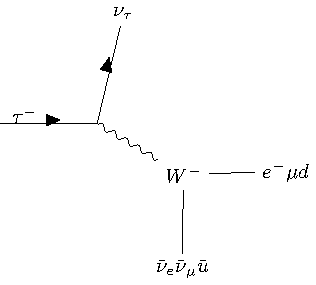
\includegraphics[width=0.35\textwidth]{"Figures/taudecay.pdf"}
    \caption{\label{fig:taudecay} diagram depicting the possible decays of the tau lepton: 65\% to a hadronic tau, 18\% to an electron, and 17\% to a muon (each with associated lepton neutrino)}
\end{center}
\end{figure} 
When the tau decays hadronically, many different intermediate mesons are produced. Each type of meson decay has a different signature, particularly when they hadronize and deposit their energy within HCAL. The Tau-POG has measured the central value systematic deviation as a form of scalar factor that is applied for an accurate result of measuring the tau's energy. This is split by the prongs (charged hadrons) and $\pi^0$ s.  

\begin{table}[h]
  \begin{center}
    \topcaption{Measured $\tauh$ energy scale correction for genuine $\tauh$'s across all years.}
    \label{tab:TES}
    \begin{tabular} { l | c  c  c }
      \hline \multicolumn{4}{c}{Correction (\%)} \\
      \hline Decay mode & 2016 & 2017 & 2018 \\ \hline
      $h^{\pm}$ & $-0.6$ & $0.7$ & $-1.3$  \\ 
      $h^{\pm}\pi^{0}$ & $-0.5$ & $-0.2$ & $-0.5$  \\ 
      $h^{\pm}h^{\pm}h^{\pm}$ & $0.0$ & $0.1$ & $-1.2$ \\ 
    \end{tabular}
  \end{center}
\end{table}

The deviation in the model is measured by taking the difference in data and MC for different values of hadronic tau energy. The uncertainty is measured for each decay mode considered in the analysis. Figures \ref{fig:taues} shows the differences in data and MC for the 1 prong + $\pi_0$ decay mode as a function of tau energy; all other tau decay modes are also measured. 

\begin{figure}[h!]
    \begin{center}
        \includegraphics[width=0.32\textwidth]{Figures/TauPOG/mtau_1ProngPi0_nominal_v3.pdf}
        \includegraphics[width=0.32\textwidth]{Figures/TauPOG/mtau_1ProngPi0_minus6percent_v3.pdf}
        \includegraphics[width=0.32\textwidth]{Figures/TauPOG/mtau_1ProngPi0_plus6percent_v3.pdf}
    \end{center}
    \caption{Tau mass distributions considering the nominal $\tau_h$ energy scale in simulation (left), or the $\tau_h$ energy scale shifted by -6 (left) or +6\% (right), in the $\mu\tau_h$ final state, for the 1 prong + $\pi^0$ decay mode.}
    \label{fig:taues}
\end{figure}

\subsection{$\tauh$ identification efficiency}

Genuine $\tauh$ identification efficiency can be different in Data and MC ~\cite{TAUIDTwiki}. To correct for this difference, measurements are 
made using genuine Z+jets production (Drell-Yan) to two $\tau$ leptons, one decays leptonically and the other hadronically. The invariant mass of the system is used as an observable. Naturally, this region has far more statistics than the control and signal regions in the pseudoscalar analysis. To measure the identification efficiency precisely, it is done in the inclusive event selection regions ~\ref{chap:selection} with an emphasis of simulation containing real taus. This measurement is done by the Tau POG, and the scale factors are provided to CMS. 
%For the $\mu\mu e \tauh$ and $\mu\mu\mu\tauh$ channels, scale factors are binned in 3 different $\pt$ bins: 30--35, 35--40, and 40+ \GeV. In the $\tauh\tauh$ final state, the efficiencies are also binned by decay mode. 

While used in the primary event and the parameter of interest in the fit, the efficiency's error is not considered in the overall systematic error as they are expected to have very little impact on fit and limits based on the 2016 result. 


\subsection{$e \rightarrow \tauh$  and $\mu \rightarrow \tauh$ misidentification rate}
The efficiency of the discriminators against electrons or muons misidentified as $\tauh$ candidates can also be different between simulation and data. 
These data/MC scale factors are
binned by barrel/endcap region of the measured $\eta(\tauh)$, and by $\tauh$ decay mode.
%Scale factors are measured to correct this difference and are applied to $e \rightarrow \tauh$ or $\mu \rightarrow \tauh$ in MC. 
Scale factors are measured to correct this difference misidentification and are applied to electrons or muons faking tau leptons in MC. 
Full information on misidentification measurements and application in analyses can be found in reference ~\cite{TAUIDTwiki}. 


The misidentification scale factors are derived by pass and fail regions. The regions are set up by selecting events where a reconstructed $\tauh$ passes the DNN working point and also fails the DNN discriminant against muons or electrons. The regions considered are QCD multijet, W+jets, and Z+jets---similar to the regions used in chapter \ref{chap:background}. QCD multijet is estimated from a same sign lepton region within data. W+Jets normalization is carefully selected from a region with high transverse mass. The visible mass distributions of the events in these regions are fit, and the overall signal yield remains constant in the pass and fail regions. 
The expected impact on the systematic error from these anti-lepton discriminators are expected to be very small so they are not included in the uncertainty model either.

%The scale factors are obtained by separating events with a reconstructed muon and a reconstructed $\tauh$ passing
%the deep tau ID into a category where the $\tauh$ passes or fails the discriminator against muons. All the processes in
%these regions are taken from simulation, except the QCD multijet background, which is estimated from SS data, and the W+jets background, which is normalized in a region with high $m_T$. The visible mass distributions in the pass and fail regions are fitted using the $e\to\tauh$ scale factor as parameter of interest. An increase of the POI causes an increase of the signal yield in the pass region and simultaneously a decrease of the signal in the fail region, such that the signal yield in the two regions combined is unchanged. 
%Additionally, the normalization of the $\PZ\to\Pe\Pe$ background is freely floating to modelna scale
%factor related to applying the discriminator against jets to muons. The scale factor applied to muons faking taus in the 
%analysis is the product of the scale factor of the discriminator against jets and scale factor of the discriminator against muons.


\subsection{Pileup re-weighting}

MC events are re-weighted using a minimum bias cross section equal to the luminosity for the corresponding year. This pileup re-weighting is to rescale the events for effective number of primary interactions during collisions. During Run II, pileup or the number of primary vertices in a crossing or underlying event could reach close to 100 and in Run III this will exceed 200.   

\subsection{Electron and muon identification efficiency}

Scale factors derived within the HTT group are applied for muons~\cite{SMHTTarXiv}, and the EGamma POG scale factors are applied for electrons~\cite{EGammaMVAID}. The scale factors for muons with $5<\pt<9$ GeV and $9<\pt<10$ GeV, are computed privately as there are no official numbers, and were approved by the MuonPOG in the 2016 analysis. These scale factors are used for the full RunII dataset. 
  
%\subsection{B tagging efficiency}

%The analysis vetoes events with at least one b tagged jet. The scale factors provided by the BTV POG~\cite{btvtwiki} are applied.

\subsection{Generator event weights and luminosity}

Generator weights are applied on an event-by-event basis. Samples produced with the aMCatNLO generator contain both positive and negative event weights. The presence of negative event weights reduces the effective yield of the samples and is included.
The event weights for simulation are scaled to the expected yields for each sample. 

To correct for differences between leading order and next to leading order cross sections, scale factors called K-factors are used. They are applied to W+Jets and Drell-Yan samples. For Drell-Yan a factor of 1.1637 is used and for W+Jets a factor of 1.221 is used.

\subsection{Low momentum muon selection}
Due to the selection of muons at 5 GeV, which is below the trigger threshold, scale factors were measured in the barrel and encaps using the tag and probe technique in the 2016 analysis. These factors are used to correct for low pt muon selection, in addition to the Muon POG's recommendation, to support correct simulation of data. 
\begin{table}[h!tbp]
\centering
\topcaption{Scale factors to correct for low momentum muon selection being less than the trigger threshold. 
\label{tab:event_yield}
}
\begin{tabular*}{0.6\textwidth}{c|c|c}
   & Barrel & Endcap \\\hline
Muons with $5 < pT < 9$ GeV & 0.956 & 0.930\\\hline
Muons with $9 < pT < 10$ GeV & 0.916 & 0.897\\\hline 
\end{tabular*}
\end{table}


\subsection{Visualizing the corrections}

The energy scales for the various leptons used in the analysis are not only changed in the nominal case, but their uncertainty is measured and then propagated to the fit model via changes in the normalization for the distribution. To visualize this and provide a cross check, distributions for the $\tau$, $\mu$, and $e$ energy scale shifts in the parameter of interest ( the mass of the di-muon system from the leading $\pt$ pseudoscalar $a$ particle) is plotted. 
These systematics for $\mu\mu\tau\tau$ channel are shown in figure \ref{fig:sys_shift_mmtt2016}.
\begin{figure}[ht!b]
  \centering
\includegraphics[width=0.31\textwidth]{Figures/outplots_v7plots_allsys_scale_m_etalt1p2Down/mll_fine_mmtt_inclusive.png} 
\includegraphics[width=0.31\textwidth]{Figures/outplots_v7plots_allsys_Nominal/mll_fine_mmtt_inclusive.png}
\includegraphics[width=0.31\textwidth]{Figures/outplots_v7plots_allsys_scale_m_etalt1p2Up/mll_fine_mmtt_inclusive.png} \\

    \caption{\label{fig:sys_shift_mmtt2016} Systematic Shift in the Uncertainty Model for 2016 $\mu\mu\tau\tau$ for the muon energy scale shift down (left), nominal (mid), and up (right), no data is shown on this plot as it directly reflects the signal region without the extraction cuts }
\end{figure}

In the end, the uncertainty considered in the fit model would then be the percent yield up and down as a flat error (log-normal) that affects the normalization of the template. Because the model is so statistically limited, the log-normal is sufficient in capturing the changes in the distributions over the fit range.  
